\documentclass{beamer}\usepackage[]{graphicx}\usepackage[]{xcolor}
% maxwidth is the original width if it is less than linewidth
% otherwise use linewidth (to make sure the graphics do not exceed the margin)
\makeatletter
\def\maxwidth{ %
  \ifdim\Gin@nat@width>\linewidth
    \linewidth
  \else
    \Gin@nat@width
  \fi
}
\makeatother

\definecolor{fgcolor}{rgb}{0.345, 0.345, 0.345}
\newcommand{\hlnum}[1]{\textcolor[rgb]{0.686,0.059,0.569}{#1}}%
\newcommand{\hlstr}[1]{\textcolor[rgb]{0.192,0.494,0.8}{#1}}%
\newcommand{\hlcom}[1]{\textcolor[rgb]{0.678,0.584,0.686}{\textit{#1}}}%
\newcommand{\hlopt}[1]{\textcolor[rgb]{0,0,0}{#1}}%
\newcommand{\hlstd}[1]{\textcolor[rgb]{0.345,0.345,0.345}{#1}}%
\newcommand{\hlkwa}[1]{\textcolor[rgb]{0.161,0.373,0.58}{\textbf{#1}}}%
\newcommand{\hlkwb}[1]{\textcolor[rgb]{0.69,0.353,0.396}{#1}}%
\newcommand{\hlkwc}[1]{\textcolor[rgb]{0.333,0.667,0.333}{#1}}%
\newcommand{\hlkwd}[1]{\textcolor[rgb]{0.737,0.353,0.396}{\textbf{#1}}}%
\let\hlipl\hlkwb

\usepackage{framed}
\makeatletter
\newenvironment{kframe}{%
 \def\at@end@of@kframe{}%
 \ifinner\ifhmode%
  \def\at@end@of@kframe{\end{minipage}}%
  \begin{minipage}{\columnwidth}%
 \fi\fi%
 \def\FrameCommand##1{\hskip\@totalleftmargin \hskip-\fboxsep
 \colorbox{shadecolor}{##1}\hskip-\fboxsep
     % There is no \\@totalrightmargin, so:
     \hskip-\linewidth \hskip-\@totalleftmargin \hskip\columnwidth}%
 \MakeFramed {\advance\hsize-\width
   \@totalleftmargin\z@ \linewidth\hsize
   \@setminipage}}%
 {\par\unskip\endMakeFramed%
 \at@end@of@kframe}
\makeatother

\definecolor{shadecolor}{rgb}{.97, .97, .97}
\definecolor{messagecolor}{rgb}{0, 0, 0}
\definecolor{warningcolor}{rgb}{1, 0, 1}
\definecolor{errorcolor}{rgb}{1, 0, 0}
\newenvironment{knitrout}{}{} % an empty environment to be redefined in TeX

\usepackage{alltt}
\mode<presentation>
{
  \usetheme{default}                    % Set theme
  \usecolortheme{default}               % Set colors
  \usefonttheme{default}                % Set font theme
  \setbeamertemplate{caption}[numbered] % Set caption to be numbered
}

\usepackage{graphicx}  % For including figures
\usepackage{booktabs}  % For table rules
\usepackage{hyperref}
\usepackage{siunitx}
\title{Exploratory Analysis of a Crime Data}  % Presentation title
\author{Team: Extra-Idiotic Family}                              % Presentation author
\institute{University of Nebraska-Lincoln}                  % Author affiliation
\date{\today}
\IfFileExists{upquote.sty}{\usepackage{upquote}}{}
\begin{document}

\begin{frame}
  \titlepage
\end{frame}


\begin{frame}{Dataset Discription}

This dataset reflects incidents of crime in the City of Los Angeles dating back to 2020. There are 521k rows (each row is a crime incident) and 28 columns (Variables)

Data set link: \href{https://data.lacity.org/Public-Safety/Crime-Data-from-2020-to-Present/2nrs-mtv8}{here}.



\begin{knitrout}
\definecolor{shadecolor}{rgb}{0.969, 0.969, 0.969}\color{fgcolor}
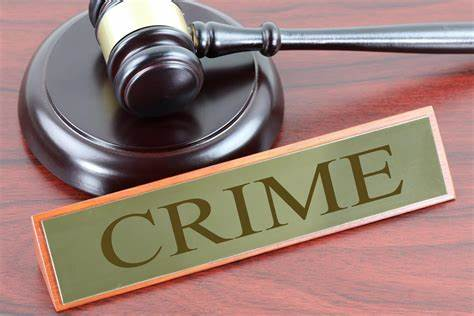
\includegraphics[width=0.5\textwidth]{figure/title.jpg}
\end{knitrout}
\end{frame}

\begin{frame}{Variables Used under Analysis}

\begin{itemize}
\item Initially there were 28 variables in the data set.
\item We focused only several variables for our analysis.
\end{itemize}



\begin{tabular}{|c||c|}
\hline
    Variable & Description \\ 
\hline
    AREA & Geographic Areas in Los-Angeles \\ 
\hline
    AREA NAME & Name designation of the area \\ 
\hline
Crm cd & crime code\\
\hline
Crm cd Desc & Defines the crime Code Provided\\
\hline
Vict Age & Age of the Victim\\
\hline
Vict Sex & Sex of the Victim\\
\hline
Vict Descent & Descent Code of the Victim\\
\hline
Premis Desc & Premises Description\\
\hline
Weapon Desc & weapon used in crime\\
\hline
\end{tabular}
\end{frame}

\begin{frame}[fragile]{Method and analysis (re-categorizing crimes)}
\begin{itemize}
\item originally there were 73 types of crime.
\item We re-categorized them as follows
\end{itemize}

\begin{knitrout}
\definecolor{shadecolor}{rgb}{0.969, 0.969, 0.969}\color{fgcolor}
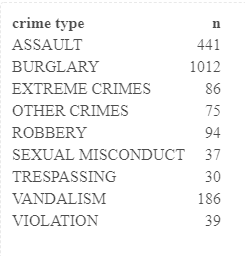
\includegraphics[width=\maxwidth]{figure/crime_types.png} 
\end{knitrout}

\end{frame}

\begin{frame}[fragile]{Method and analysis (Cleaning Age variable)}
\begin{columns}
		\column{.6\textwidth}
\begin{knitrout}
\definecolor{shadecolor}{rgb}{0.969, 0.969, 0.969}\color{fgcolor}
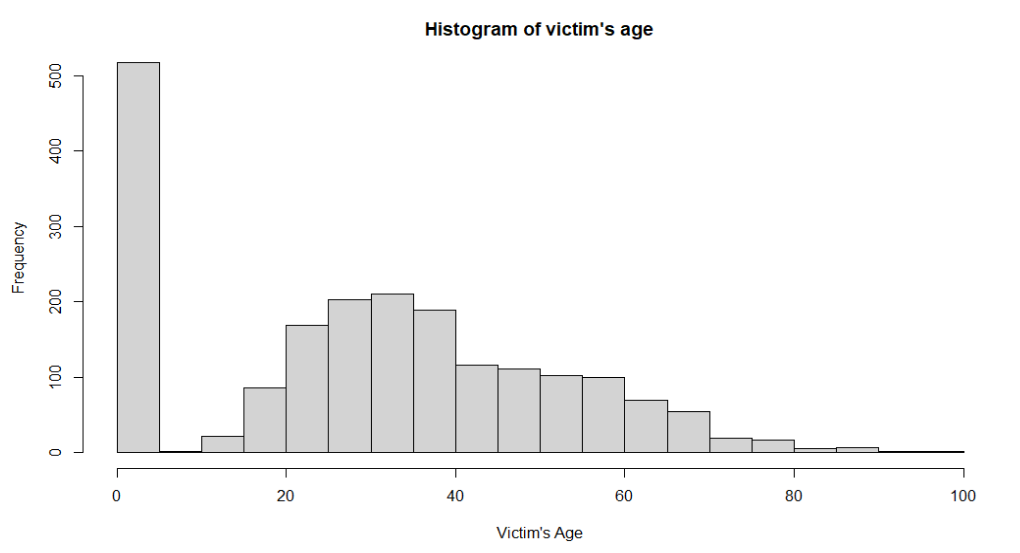
\includegraphics[width=\maxwidth]{figure/hist_age.png} 
\end{knitrout}

\column{.4\textwidth}
\textbf{Highlights}
\begin{itemize}
\item Unusual number of Zero records.
\item replace them with median of age. 
\item continue the analysis.

\end{itemize}

\end{columns}
\end{frame}

\begin{frame}[fragile]{Method and analysis (Re-categorizing Descent variable)}
\begin{columns}
		\column{.5\textwidth}
\begin{knitrout}
\definecolor{shadecolor}{rgb}{0.969, 0.969, 0.969}\color{fgcolor}
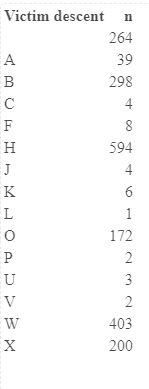
\includegraphics[width=\maxwidth]{figure/Des_categories.png} 
\end{knitrout}

\column{.5\textwidth}
\begin{tabular}{|c||c|}
\hline
    Symbol & Descecnt \\ 
\hline
    A & Other Asian \\ 
\hline
    B & Black \\ 
\hline
H & Hispanic/Latin/Mexican\\
\hline
O & other\\
\hline
W & white\\
\hline
 & Minor or Unknown\\
\hline

\end{tabular}

\end{columns}
\end{frame}

\begin{frame}[fragile]{Relationship with the area and the crime}

which area is the most awfull to live.

\begin{knitrout}
\definecolor{shadecolor}{rgb}{0.969, 0.969, 0.969}\color{fgcolor}
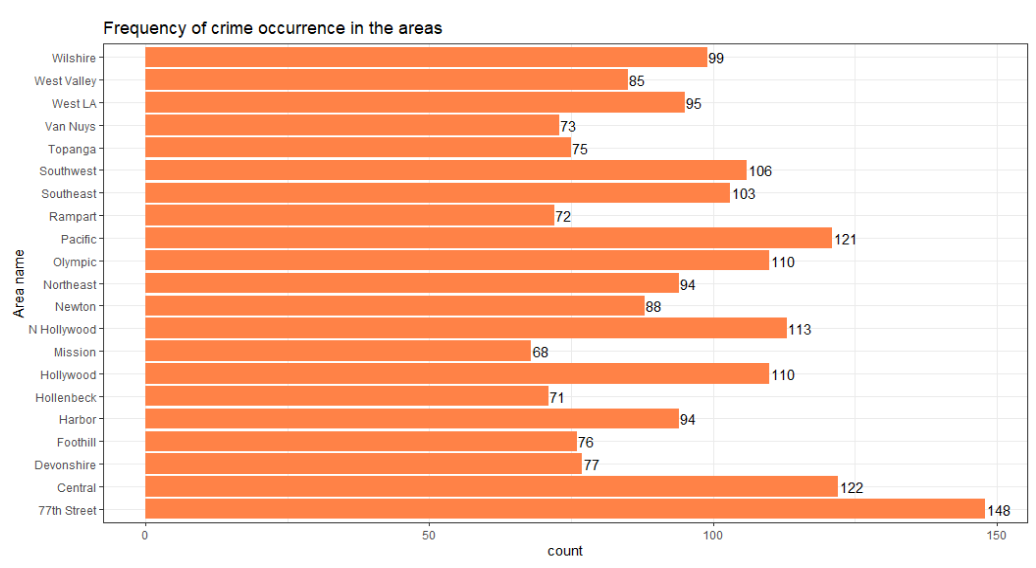
\includegraphics[width=\maxwidth]{figure/place.png} 
\end{knitrout}
\textbf{Highlights}
\begin{itemize}
\item 77th street has the highest number of crimes.
\item 100+ crimes have been reported over some other areas
\item Please avoid those areas.

\end{itemize}
\end{frame}

\begin{frame}[fragile]{Which type of crimes ocured most}
\begin{columns}
		\column{.5\textwidth}
\begin{knitrout}
\definecolor{shadecolor}{rgb}{0.969, 0.969, 0.969}\color{fgcolor}
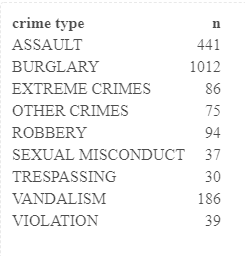
\includegraphics[width=\maxwidth]{figure/crime_types.png} 
\end{knitrout}

\column{.5\textwidth}
\textbf{Highlights}
\begin{itemize}
\item Burglary And Assault
\begin{knitrout}
\definecolor{shadecolor}{rgb}{0.969, 0.969, 0.969}\color{fgcolor}
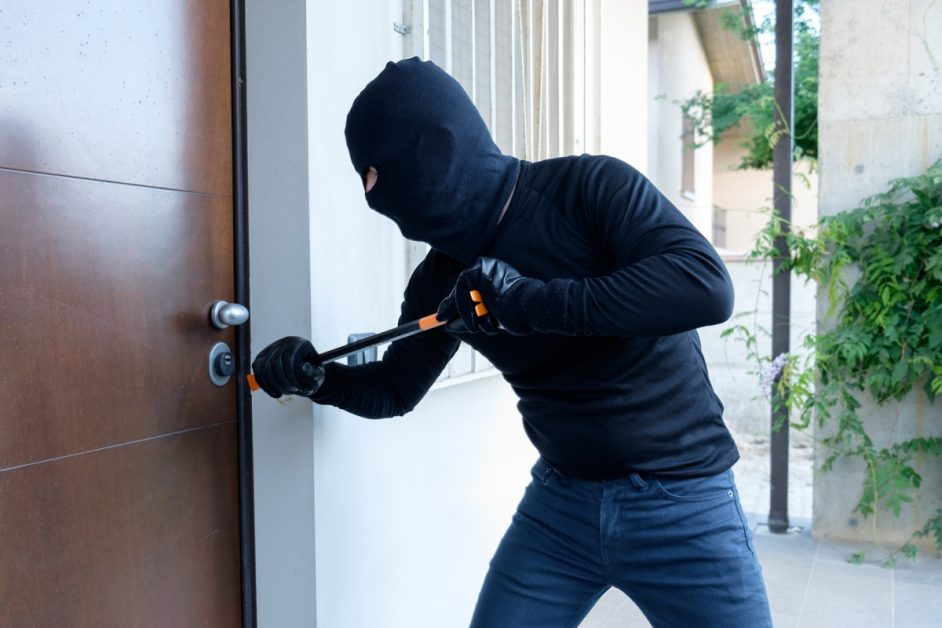
\includegraphics[width=\maxwidth]{figure/bur.jpg} 
\end{knitrout}
\begin{knitrout}
\definecolor{shadecolor}{rgb}{0.969, 0.969, 0.969}\color{fgcolor}
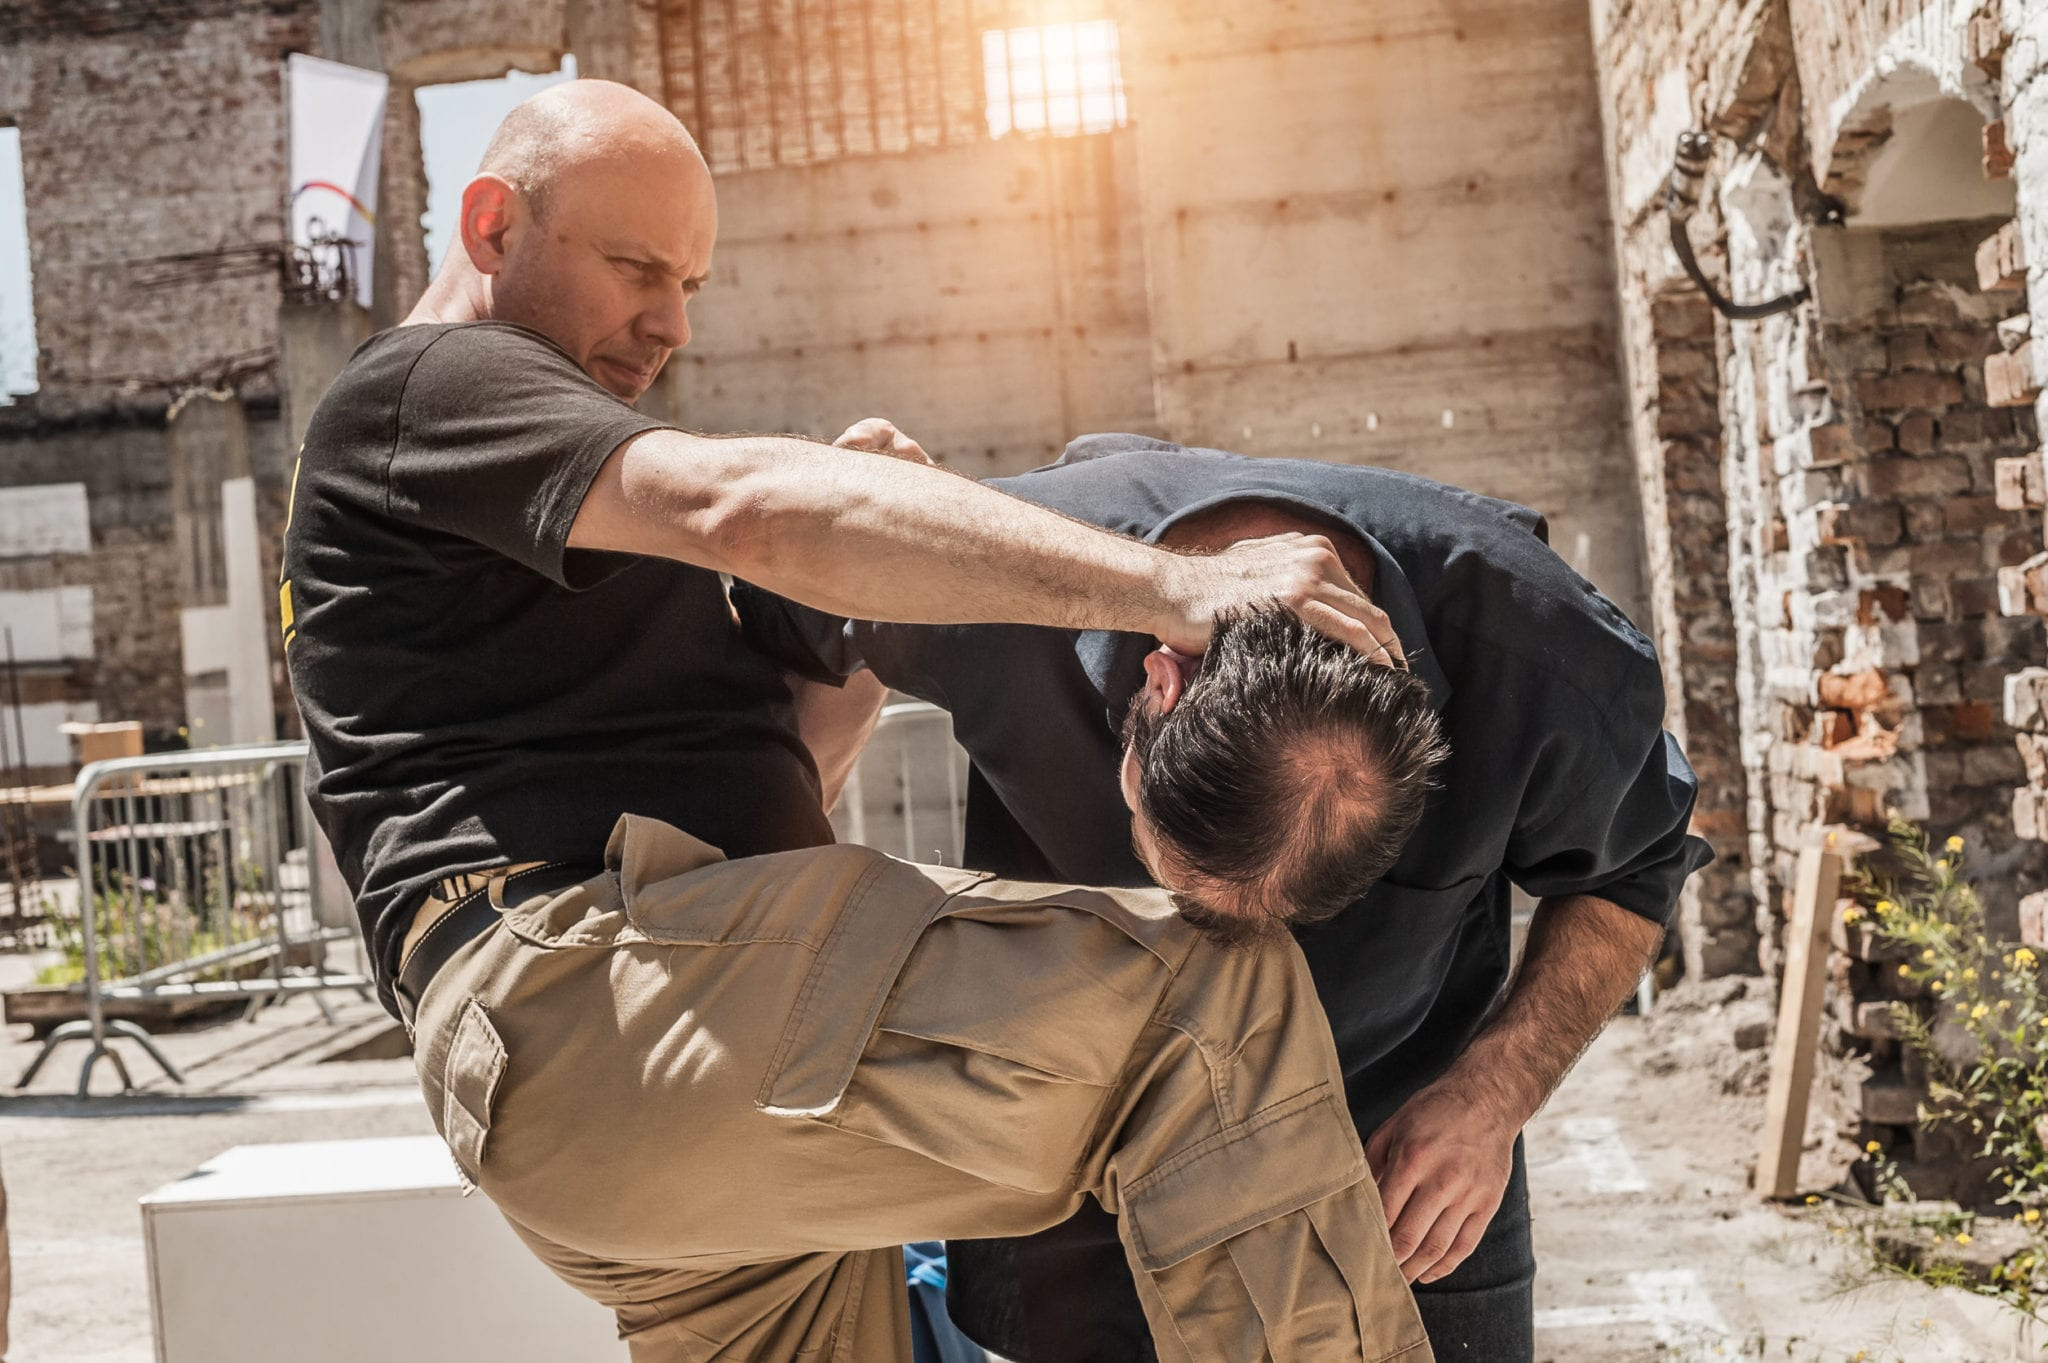
\includegraphics[width=\maxwidth]{figure/as.jpg} 
\end{knitrout}
\end{itemize}

\end{columns}
\end{frame}

\begin{frame}[fragile]{Relationship between the area and the crime "Assault"}

\begin{knitrout}
\definecolor{shadecolor}{rgb}{0.969, 0.969, 0.969}\color{fgcolor}
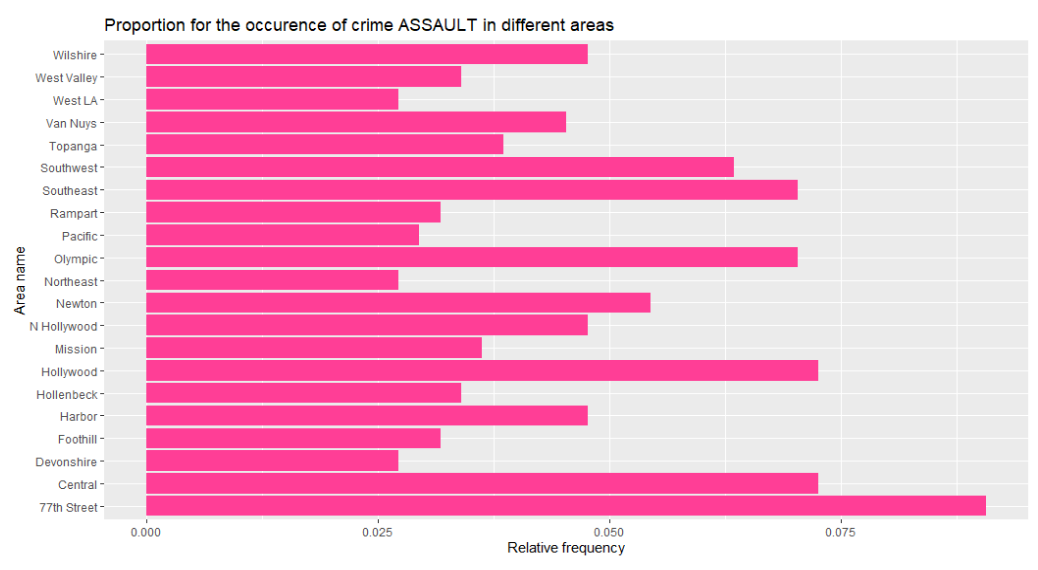
\includegraphics[width=\maxwidth]{figure/assault.png} 
\end{knitrout}
\textbf{Highlights}
\begin{itemize}
\item 77th street 
\item Southeast, Olymic, Hollywood, Central

\end{itemize}
\end{frame}

\begin{frame}[fragile]{Relationship between the area and the crime "Burglary"}

\begin{knitrout}
\definecolor{shadecolor}{rgb}{0.969, 0.969, 0.969}\color{fgcolor}
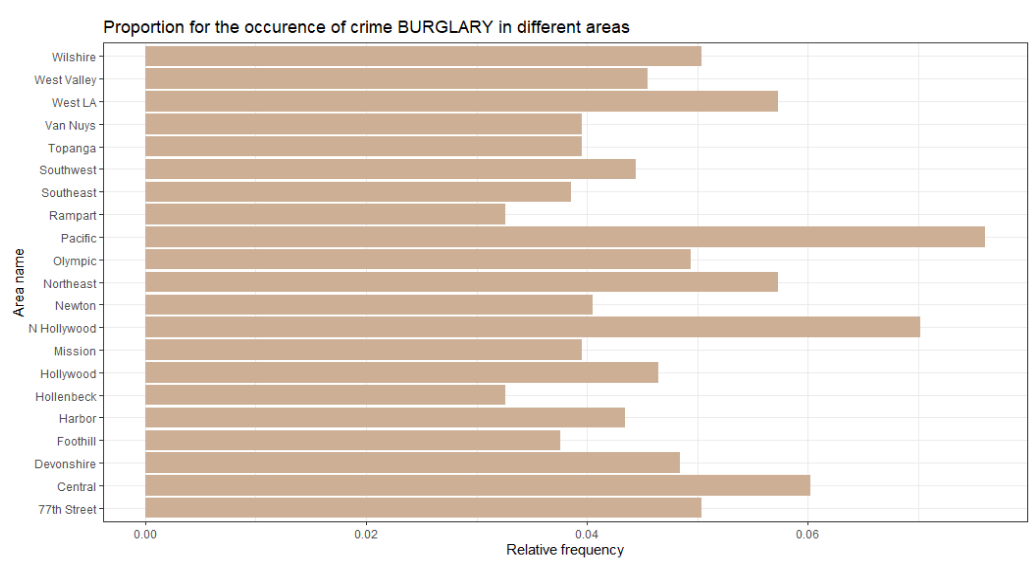
\includegraphics[width=\maxwidth]{figure/burglary.png} 
\end{knitrout}
\textbf{Highlights}
\begin{itemize}
\item Pacific 
\item West LA, Northeast, N Hollywood, Central

\end{itemize}
\end{frame}

\begin{frame}[fragile]{Relationship between the age and the crime type}

\begin{knitrout}
\definecolor{shadecolor}{rgb}{0.969, 0.969, 0.969}\color{fgcolor}
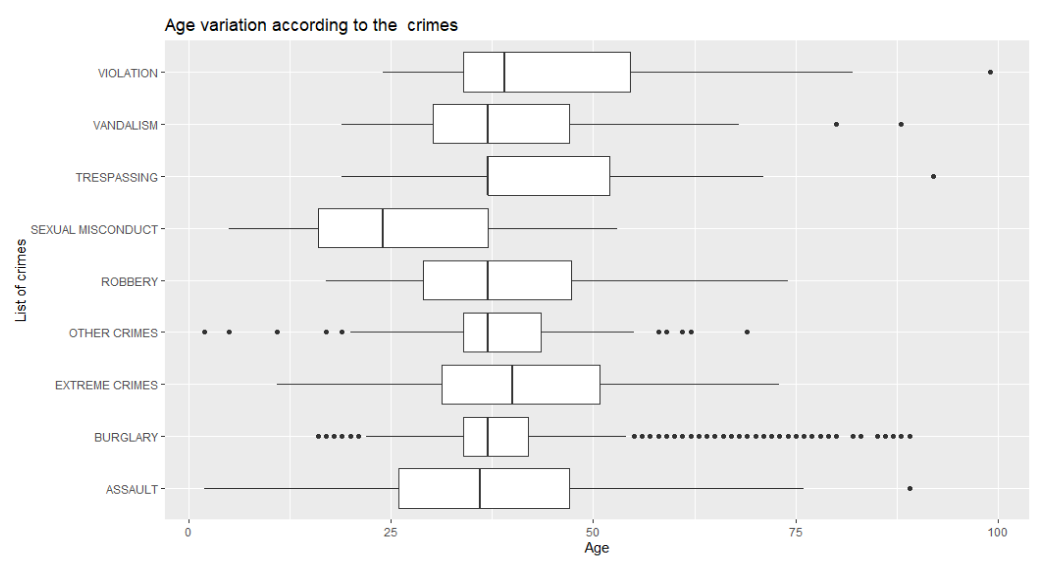
\includegraphics[width=\maxwidth]{figure/box_age.png} 
\end{knitrout}
\textbf{Highlights}
\begin{itemize}
\item From the IQR we can roughly say majority of victims are in between 25 and 50 for all the crimes except the sexual misconduct.

\end{itemize}
\end{frame}

\begin{frame}[fragile]{Relationship between the Descent and the crime type}

\begin{knitrout}
\definecolor{shadecolor}{rgb}{0.969, 0.969, 0.969}\color{fgcolor}
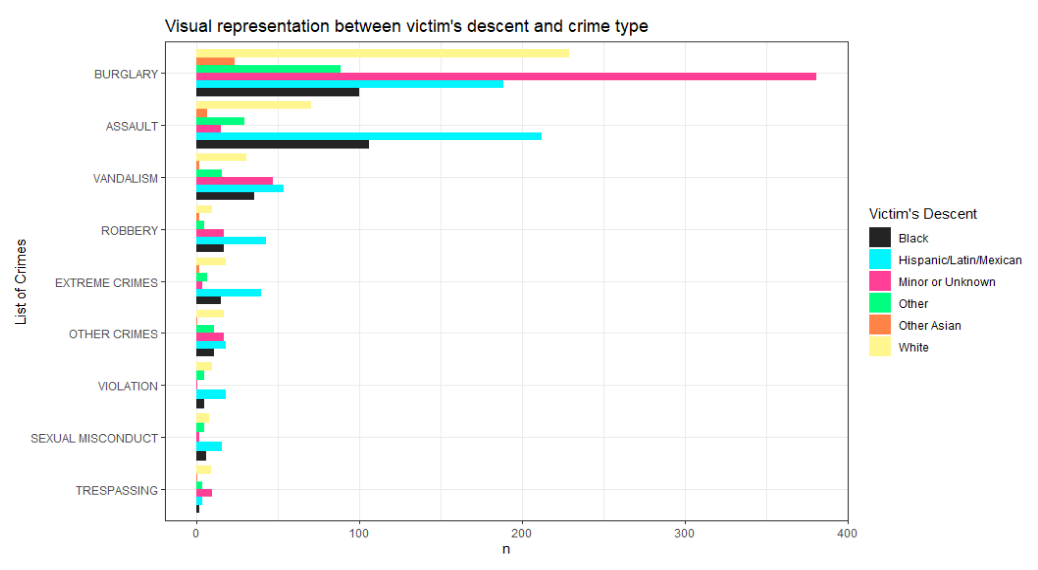
\includegraphics[width=\maxwidth]{figure/descent.png} 
\end{knitrout}
\textbf{Highlights}
\begin{itemize}
\item Hispanic/Latin/Mexican have faced every type of crime more except for the burglary
\item Burglary is faced by White people more.
\item Assault is faced by a considerable number of black people
\end{itemize}
\end{frame}



\begin{frame}[fragile]{Crime and Victim's Sex}

\begin{itemize}
\item Explore which sex groups are facing which type of crime more.
\item The variable victim's sex was coded as Male, Female, and Unknown (Missing or reported as unknown).

\end{itemize}


\end{frame}

\begin{frame}[fragile]{Answer to Crime and Victim's Sex}
\begin{columns}
		\column{.6\textwidth}
\begin{knitrout}
\definecolor{shadecolor}{rgb}{0.969, 0.969, 0.969}\color{fgcolor}
\includegraphics[width=\maxwidth]{figure/unnamed-chunk-2-1} 
\end{knitrout}

\column{.4\textwidth}
\textbf{Highlights}
\begin{itemize}
\item Burglary, assault, vandalism, robbery and extreme crimes are mostly happening with the males.
\item Females are more victim of violation and sexual misconduct compared to males. 
\item Crimes other than the specified ones are occurring both equally.

\end{itemize}

\end{columns}
\end{frame} 


\begin{frame}[fragile]{Premises of crime}

\begin{itemize}
\item Explore the premises of different crimes we defined.
\item We are reporting the premises which appeared more than 3\% of the times for the crimes.

\end{itemize}

\end{frame}

\begin{frame}[fragile]{Premises of Burglary}
\begin{knitrout}
\definecolor{shadecolor}{rgb}{0.969, 0.969, 0.969}\color{fgcolor}
\begin{tabular}{l}
\hline
Premises of Burglary\\
\hline
DRIVEWAY\\
\hline
GARAGE/CARPORT\\
\hline
MULTI-UNIT DWELLING (APARTMENT, DUPLEX, ETC)\\
\hline
OTHER BUSINESS\\
\hline
PARKING LOT\\
\hline
SINGLE FAMILY DWELLING\\
\hline
STREET\\
\hline
\end{tabular}

\end{knitrout}
\vspace{0.5cm}
\textbf{Highlights}: Driveway, garage, multi-unit or single family dwelling, street, parking lot are the frequently occurred premises for the crime burglary.

\end{frame}


\begin{frame}[fragile]{Premises of Assault}
\begin{knitrout}
\definecolor{shadecolor}{rgb}{0.969, 0.969, 0.969}\color{fgcolor}
\begin{tabular}{l}
\hline
Premis of Assault\\
\hline
MULTI-UNIT DWELLING (APARTMENT, DUPLEX, ETC)\\
\hline
PARKING LOT\\
\hline
SIDEWALK\\
\hline
SINGLE FAMILY DWELLING\\
\hline
STREET\\
\hline
\end{tabular}

\end{knitrout}
\vspace{0.5cm}
\textbf{Highlights}: Assault is being reported frequently taking place in street, sidewalk, parking lot, and single family or multi-unit dwelling.
\end{frame}

\begin{frame}[fragile]{Premis of Sexual Misconduct}

\begin{knitrout}
\definecolor{shadecolor}{rgb}{0.969, 0.969, 0.969}\color{fgcolor}
\begin{tabular}{l}
\hline
Premis of Sexual Misconduct\\
\hline
MULTI-UNIT DWELLING (APARTMENT, DUPLEX, ETC)\\
\hline
OTHER BUSINESS\\
\hline
POLICE FACILITY\\
\hline
SIDEWALK\\
\hline
SINGLE FAMILY DWELLING\\
\hline
STREET\\
\hline
\end{tabular}

\end{knitrout}
\vspace{0.5cm}
\textbf{Highlights}: Sexual misconduct is similar to the premises that were reported for burglary and assault but the interesting is that we found that \textbf{police facility} is a frequently occurred premise.
\end{frame}


\begin{frame}[fragile]{Premis of Extreme Crimes}

\begin{knitrout}
\definecolor{shadecolor}{rgb}{0.969, 0.969, 0.969}\color{fgcolor}
\begin{tabular}{l}
\hline
Premis of Extreme Crimes\\
\hline
ALLEY\\
\hline
MULTI-UNIT DWELLING (APARTMENT, DUPLEX, ETC)\\
\hline
PARKING LOT\\
\hline
SIDEWALK\\
\hline
SINGLE FAMILY DWELLING\\
\hline
STREET\\
\hline
\end{tabular}

\end{knitrout}
\vspace{0.5cm}
\textbf{Highlights}: Alley is a new premise we observed in case of extreme crimes and rest of the premises are same as observed for previous crimes. 
\end{frame}


\begin{frame}[fragile]{Weapons used in crime}


\begin{itemize}
\item we explored whether for committing a particular type of crime commit-er has preference over the weapons based on the victim's sex.

\item We reported the weapons used more than 10 times for committing a particular crime in the data-set.
\end{itemize}


\end{frame}

\begin{frame}[fragile]{Answer to weapons used in Assault}
\begin{knitrout}
\definecolor{shadecolor}{rgb}{0.969, 0.969, 0.969}\color{fgcolor}
\includegraphics[width=\maxwidth]{figure/unnamed-chunk-7-1} 
\end{knitrout}



\end{frame}


\begin{frame}[fragile]{Answer to weapons used in sexual misconduct}
\begin{knitrout}
\definecolor{shadecolor}{rgb}{0.969, 0.969, 0.969}\color{fgcolor}
\includegraphics[width=\maxwidth]{figure/unnamed-chunk-8-1} 
\end{knitrout}
\end{frame}


\begin{frame}[fragile]{Current status of the crimes}


\begin{itemize}
\item We explored which type of crimes are getting resolved mostly and which type are not

\item We re-categorized the variable indicating case status into "Not Resolved" if the investigation is continued otherwise coded as "Resolved".
\end{itemize}
\end{frame}



\begin{frame}[fragile]{Answer to status of the crimes}
\begin{columns}
		\column{.55\textwidth}
\begin{knitrout}
\definecolor{shadecolor}{rgb}{0.969, 0.969, 0.969}\color{fgcolor}
\includegraphics[width=\maxwidth]{figure/unnamed-chunk-9-1} 
\end{knitrout}

\column{.45\textwidth}
\textbf{Highlights}
\begin{itemize}
\item The crime violation is getting resolved more than any any other crimes in the data-set.
\item Trespassing, burglary, robbery, and sexual misconduct has a fairly large difference between proportion of resolved and not resolved cases. 
\item Assault and extreme crime has shorter difference between proportion resolved and not resolved.

\end{itemize}

\end{columns}
\end{frame} 



\end{document}
